\documentclass[final]{article}


\usepackage{aps360}             % course style file (file name is lower case: aps360.sty)
\usepackage[utf8]{inputenc} % allow utf-8 input
\usepackage[T1]{fontenc}    % use 8-bit T1 fonts
\usepackage[colorlinks=true,linkcolor=black,citecolor=blue!50!black,urlcolor=blue!50!black]{hyperref}
\usepackage{url}            % simple URL typesetting
\usepackage{booktabs}       % professional-quality tables
\usepackage{amsfonts}       % blackboard math symbols
\usepackage{amsmath}
\usepackage{nicefrac}       % compact symbols for 1/2, etc.
\usepackage{microtype}      % microtypography
\usepackage{xcolor}         % colors
\usepackage{graphicx}

% The [final] option of aps360.sty prints a NeurIPS track name in the first-page
% footer, but no track is defined, which causes an "Undefined control sequence"
% error. Leave the footer empty instead.
\makeatletter
\renewcommand{\@noticestring}{}
\makeatother

\title{Hearing Risk: Predicting Post-Earnings\\Stock Volatility from Executive Speech}

\author{%
  First \& Last Name \\
  Student Number, email@mail.utoronto.ca\\
  GitHub: \url{https://github.com/USERNAME/REPO}\\
}

\begin{document}

\maketitle

\vspace{-0.45in}

\section*{Introduction}
After a company reports earnings, its stock price often becomes much more volatile for days or weeks.
Volatility drives option prices, value-at-risk limits and portfolio hedging, so forecasting it well has
direct value for risk managers. In the live earnings call, executives answer unscripted analyst
questions, and listeners pick up on hesitation, stress and confidence that a written transcript does not record.
This project asks: \emph{does how executives speak in the Q\&A section of an earnings call predict
post-call realized volatility, beyond what past volatility and the transcript text already explain?}
The goal is a model that takes a call's audio and transcript and predicts log realized volatility
over the next 3, 7, 15 and 30 trading days.
Deep learning is a natural fit because the input is raw, high-dimensional speech: the useful cues
(pitch movement, pauses, speaking rate, energy) are not known in advance and must be learned from
spectrograms, and a call contains hundreds of sentences whose importance varies, which an attention
mechanism can learn to weigh. Hand-crafted features and linear models serve as the point of comparison.

\section*{Illustration}
Figure~\ref{fig:pipeline} shows the proposed model. Each executive sentence is encoded twice, from its
audio clip and from its text, the two vectors are fused, and the call is summarized by attention pooling
before a regression head that also sees past volatility.

\begin{figure}[!h]
  \centering
  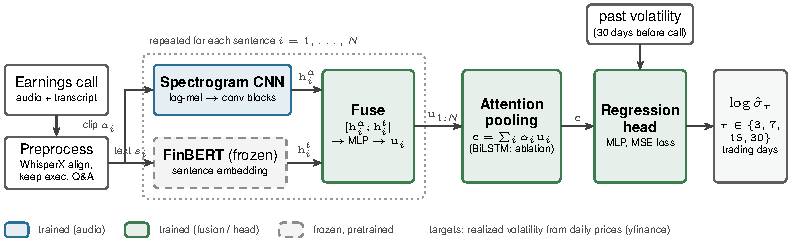
\includegraphics[width=\linewidth]{figures/pipeline.pdf}
  \caption{Proposed pipeline. Audio and text are encoded per sentence, fused, pooled over the call, and
  combined with past volatility to predict log realized volatility at four horizons.}
  \label{fig:pipeline}
\end{figure}

\vspace{-0.1in}
\section*{Background \& Related Work}
\citet{kogan2009predicting} first showed that text (10-K reports) predicts future volatility beyond
past volatility, using linear regression on word features. \citet{qin2019what} introduced the
earnings-call dataset used here and a multimodal deep regression model (MDRM) with BiLSTMs over
sentence-level text and 27 hand-crafted vocal features, finding that vocal cues improve volatility
prediction. \citet{yang2020html} replaced the BiLSTM with a hierarchical transformer and multi-task
learning, and \citet{sawhney2020voltage} added a graph network over related stocks (VolTAGE).
\citet{li2020maec} released MAEC, a larger aligned earnings-call dataset for S\&P~1500 firms.
Most recently, \citet{chen2025sound} found that acoustic and textual features do not predict the
direction of returns but explain up to 43.8\% of out-of-sample variance in 30-day realized volatility, and
\citet{shu2026fincall} released FinCall-Surprise, 2,688 calls with full audio, transcripts and slides.
Nearly all prior work describes audio with a fixed set of hand-crafted features (e.g., openSMILE
\citep{eyben2010opensmile}). This project instead learns the audio representation directly from
spectrograms and compares it with pretrained speech features \citep{baevski2020wav2vec}.

\section*{Data Processing}
\textbf{Sources.} (1) MDRM \citep{qin2019what}: about 570 S\&P~500 calls from 2017, already split into
sentence-level audio clips aligned with transcript sentences. (2) FinCall-Surprise \citep{shu2026fincall}:
2,688 calls from 2019--2021 with full-length audio and transcripts. (3) Daily adjusted closing prices from
Yahoo Finance (\texttt{yfinance}).
\textbf{Steps.} (i) Resample all audio to 16\,kHz mono. (ii) For FinCall-Surprise, split transcripts into
sentences and force-align them to the audio with WhisperX \citep{bain2023whisperx} to obtain one clip per
sentence; discard sentences with low alignment confidence. (iii) Using the transcript speaker headers, keep
only executive sentences from the Q\&A section, and apply the same rule to MDRM so both sources share
one pipeline. Drop calls with fewer than 20 usable sentences. (iv) Convert each clip to a 64-band
log-mel spectrogram (25\,ms window, 10\,ms hop), crop or pad to 8\,s, and normalize with training-set
statistics. (v) Compute and cache frozen FinBERT \citep{araci2019finbert} embeddings for every sentence.
(vi) Labels: with daily log returns $r_t$, $v_{\tau} = \ln\sqrt{\tfrac{1}{\tau}\sum_{t=1}^{\tau}(r_t-\bar r)^2}$
for $\tau \in \{3,7,15,30\}$, where day~1 is the first full trading day after the call (next day for
after-close calls). Past volatility uses the same formula over the 30 days before the call. Calls with
missing prices (e.g., delisted tickers) are dropped.
\textbf{Split.} Chronological, to avoid look-ahead: train 2017--2019, validation 2020, test 2021. Because
2020 was an unusual COVID volatility period, results will also be reported with it excluded.

\section*{Architecture}
\textbf{Audio branch:} a CNN trained from scratch on spectrograms (4 blocks of $3\times3$ conv,
batch norm, ReLU and $2\times2$ max-pooling; 16--128 channels), followed by global average pooling to a
128-d vector $\mathbf{h}^a_i$. \textbf{Text branch:} the frozen FinBERT embedding projected to 128-d,
$\mathbf{h}^t_i$. \textbf{Fusion:} $\mathbf{u}_i = \mathrm{MLP}([\mathbf{h}^a_i;\mathbf{h}^t_i])$.
\textbf{Call level:} attention pooling $\mathbf{c} = \sum_i \alpha_i \mathbf{u}_i$ with
$\alpha_i = \mathrm{softmax}_i(\mathbf{w}^\top \tanh(W\mathbf{u}_i))$; a BiLSTM over the sentence
sequence is a comparison. \textbf{Head:} an MLP on $[\mathbf{c}; \text{past vol.}]$ outputs the four
$v_\tau$, trained with mean MSE using Adam, dropout and early stopping on validation loss.
Planned comparisons: wav2vec~2.0 features in place of the CNN, and text-only, audio-only and
audio+text ablations. Success is measured by test MSE and $R^2$ at each horizon relative to the baselines.

\section*{Baseline Model}
(1) \textbf{Past volatility only:} ordinary least squares $v_\tau = a_\tau + b_\tau\,v_{\text{past}}$
fitted on the training years. Volatility is highly persistent, so this is the bar the network must beat;
GARCH(1,1) \citep{bollerslev1986garch} is an optional second version.
(2) \textbf{Hand-crafted vocal features:} the 88 openSMILE eGeMAPS features (pitch, jitter, shimmer,
loudness, speech rate) per sentence, averaged over the call, plus past volatility, fed to ridge regression
with the penalty tuned on validation data.

\section*{Ethical Considerations}
Vocal features can carry accent, gender, age and non-native-speaker traits; a model that links these to
``risk'' could unfairly penalize some executives and their firms, so errors will be compared across
available speaker groups. Executives could also be coached to game such a model. The data covers only
large U.S. firms and three years, so results may not generalize, and the model is a research tool,
not trading advice; deploying it for automated trading without that context could cause financial harm.
Recordings are public, but they still contain identifiable voices and will not be redistributed.

\newpage
\bibliographystyle{plainnat}
\bibliography{references}

\end{document}
